\chapter{Functional}

Functional refers to a mapping of functions or curves (belonging to a certain set) to a definite number. From this perspective, functional can be regarded as an extension to function. Functional has many practical applications in analysis, mechanics, geometry, control systems, etc. Many optimization problems are defined using functional.

It is worth mentioning here the relationship between functional and calculus of variation. Assume $y(x)$ a function of $x$. Let $F$ be a deterministic function of $x$ and $y$, for example, $F(x, y, y\prime)$. The study of
\begin{eqnarray}
	J = \int_{a}^{b} F dx \nonumber
\end{eqnarray}
with different choice of $y(x)$ is called ``calculus of functional''.

Calculus of functional is often difficult to solve. Calculus of variation is a special case of calculus of functional that only studies the behavior of $y$ when $J$ is at its maximum or minimum value. A typical example of calculus of vibration is, for example, to find $y$ that minimizes $J$.

Though simplified comparing with calculus of functional, calculus of variation is still difficult to solve in general. Its analytical solution exists for only certain forms of $F$.

\section{A Motivating Example}

One of the most famous problems solved by functional and calculus of variation is the brachistochrone problem. The description to the problem is given in the box.

\begin{shortbox}
\Boxhead{Brachistochrone Problem}

Let A and B be two fixed points in a vertical plane, where A is higher than B (from gravity perspective) and A, B are not aligned vertically. Draw a curve that joins A and B. A particle is released from A and it slides along the curve traveling from A to B driven by gravity, hence its velocity decided by the position of the particle (speed) and the tangent of the curve at the particle position (direction). A demonstration is given by Fig. \ref{ch12fig:brachistochrone_description}.

The brachistochrone problem tries to find the curve that minimizes the time it takes for the particle to travel from A to B. The objective is to find the analytical solution $y=f(x)$ that describes such curve.

\end{shortbox}

\begin{figure}
	\centering
	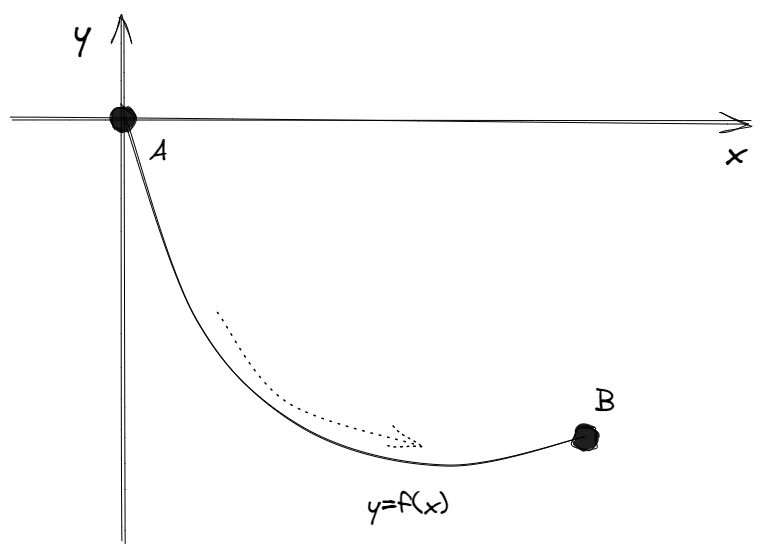
\includegraphics[width=200pt]{chapters/chapter12/figures/brachistochrone_description.png}
	\caption{Brachistochrone problem description.} \label{ch12fig:brachistochrone_description}
\end{figure}

\section{Functional}

\section{Commonly Seen Functional Examples}

